\documentclass[12pt]{article}
\usepackage{amsmath,amssymb,amsthm,amsfonts}
\usepackage{multicol}
\usepackage{color}
\usepackage{hyperref}
\usepackage{graphicx}

\newcommand{\co}[1]{\stackrel{\circ }{#1}}
\newcommand{\gf}{\mathfrak{g}}
\newcommand{\nfp}{\mathfrak{n}^{+}}
\newcommand{\nfm}{\mathfrak{n}^{-}}
\newcommand{\af}{\mathfrak{a}}
\newcommand{\uf}{\mathfrak{u}}
\newcommand{\sfr}{\mathfrak{s}}
\newcommand{\aft}{\widetilde{\mathfrak{a}}}
\newcommand{\afb}{\mathfrak{a}_{\bot}}
\newcommand{\hf}{\mathfrak{h}}
\newcommand{\hfb}{\mathfrak{h}_{\bot}}
\newcommand{\pf}{\mathfrak{p}}

\newcommand{\gfh}{\hat{\mathfrak{g}}}
\newcommand{\afh}{\hat{\mathfrak{a}}}
\newcommand{\sfh}{\hat{\mathfrak{s}}}
\newcommand{\bff}{\mathfrak{b}}
\newcommand{\hfg}{\hf_{\gf}}

\begin{document}
\title{Schramm-Loewner evolution in tricritical Ising model}

\maketitle

Tricritical Ising: integrability (RSOS), supersymmetry (?), conformally-invariant boundary conditions, identification with CFT. 
CFT with supersymmetry (additional generators and relations). 
Boundary conditions, CFT primary fields and SLE. 
SLE on superspace \cite{nagi2005stochastic,rasmussen2004stochastic} and BCFT for tricritical Ising (parameter correspondence).

Proof: discrete holomorphicity and integrability. 
(Loop description?)

\section{Tricritical Ising model: definition}
\label{sec:tricr-ising-model}

The 2-Dimensional tricritical Ising model is the simplest known statistical model to exhibit
supersymmetry. This simple model has a long history of theoretical and experimental study.

Several lattice realization of tricritical Ising model are possible. We consider the dilute Ising model and the $A_4$
Restricted Solid-on-Solid (RSOS) model. The dilute Ising model has the classical Hamiltonian 
\begin{equation}
  \label{eq:1}
  H = -\beta \sum_{<i,j>}\sigma_i\sigma_j - \mu \sum_{i}(\sigma_i)^2  
\end{equation}
where $i,j$ label the lattice sites, each of the variables $\sigma_i$
takes three values $-1,0,1$ ($0$ represents the vacant site) and the
first sum in (\ref{eq:1}) is made over nearest neighbor pairs. Concentration
of the vacancies is controlled by the chemical potential $\mu$. The
phase diagram of this system in coordinates of temperature $T$ and
$e^{-\mu}$ is shown in Fig.~\ref{fig:phase-diagram}.

\begin{figure}[h]
  \centering{
    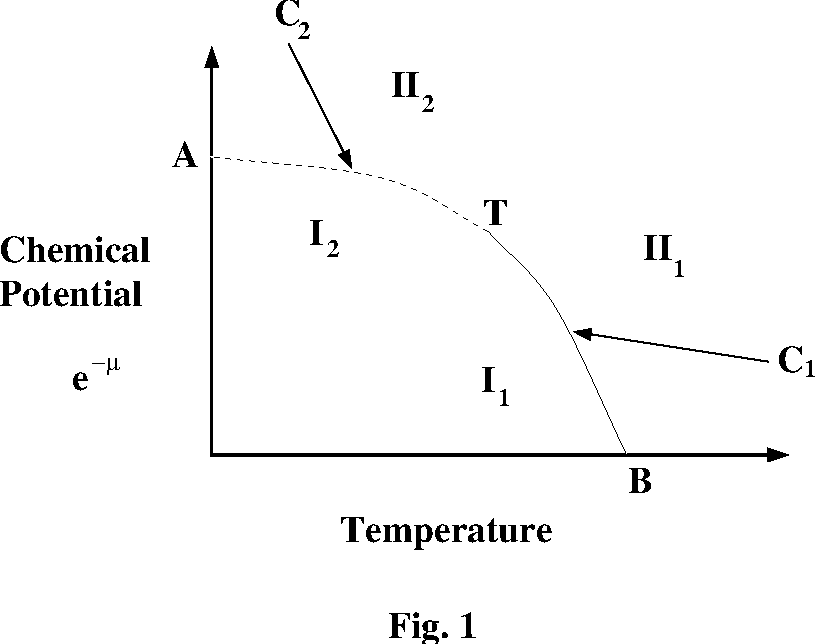
\includegraphics[height=70mm]{fig1}
    \caption{Phase diagram for the dilute Ising model}}
  \label{fig:phase-diagram}
\end{figure}


 There are two phases
separated by a line AB of phase transition. For low vacancies and low
temperature, we have an ordered phase I with spontaneously broken $Z_2$
symmetry. On the other side of the transition line we have a disordered
phase II with unbroken symmetry. The point B is the usual critical point
of the Ising model, and the solid segment BT corresponds to the second
order transition belonging to the Ising model universality class. The
dotted segment AT is a line of first order phase transition. The point T
where the two critical segments joined smoothly is the tricritical point of the
system. 
%%  
%%  This model belongs to the universality class of the
%%  Landau-Ginzburg $\varphi^6$-theory at this tricritical point [23], so
%%  the phase diagram could also be understood in terms
%%  of the Landau-Ginzburg effective potential of this system [14].
%%  This effective potential (specific free energy) is plotted
%%  as the function of the order parameter ($<\sigma>$) of this system in Fig.2
%%  for various regions of the phase diagram.
%%  The ground state is degenerate in phase I,
%%  while in phase II it is non-degenerate. There is only one vacuum
%%  on the line BT, typical of a second order transition.
%%  Note that along the first
%%  order transition line AT, the vacuum is in fact three-fold degenerate.
%%


\section{Restricted solid on solid models}
\label{sec:restr-solid-solid}

The $A_4$ RSOS lattice realization of tricritical Ising models is constructed as follows.
Consider a diagonal square lattice where the degree of
freedom at each site can take on four values $l_i = 1, 2, 3, 4$.
The value of $l_i$ is further constrained by the requirement
$|l_i-l_j| = 1$ for nearest neighbor sites $i$ and $j$. We can say
that possible spin values are labeled by nodes of $A_4$ Dynkin
diagram and neighboring spins are labeled by connected nodes.

There is a ferromagnetic next-nearest-neighbor interaction and a
single-site interaction. The lattice can be divided into two sublattices
I and II, where the values of $l_i$ are odd in one sublattice, and
even in the other sublattice. There are three degenerate
ground states as shown in Fig.~\ref{fig:vacua}.
\begin{figure}[h]
  \centering{
    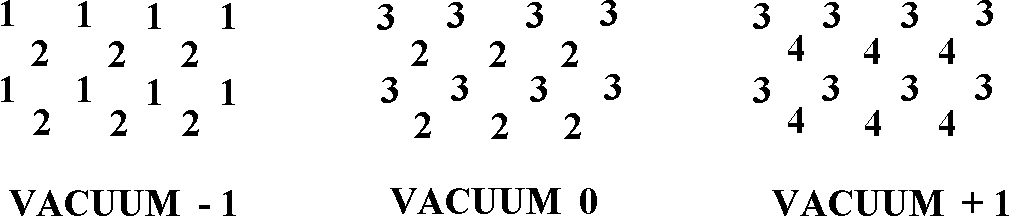
\includegraphics[width=90mm]{vacua}
    \caption{Vacua for $A_4$ RSOS model}}
  \label{fig:vacua}
\end{figure}


To make contact with the order parameter $<\sigma>$ of the Ising model
with vacancies (\ref{eq:1}),  the ground states are labeled by $-1, 0$
and $+1$ in Fig.~\ref{fig:vacua} \cite{chim1996boundary}.



The Hamiltonian of the RSOS model is symmetric under
the global $Z_2$ transform $l_i \to 5 - l_i$, which corresponds to the
spin-reversal symmetry of the model (1). The three ground states will
become identical in the bulk at the tricritical point. However the nature
of the order parameter at the boundary will depend on the specific boundary
condition. As shown in [2], the state $|\tilde{\Delta}_{(1,s)}\rangle$ corresponds
to the
boundary condition where all boundary degrees of freedom are fixed to the
value $s$, this is illustrated in Fig.10.
For the state $|\tilde{0}\rangle$, the boundary degrees of freedom are fixed to
$1$, and hence the neighboring state must be in the state $2$. Thus in
the continuum limit, the order parameter at the boundary will be in the $-1$
vacuum, and we shall denote this boundary condition by $(-)$. The boundary
state $|\tilde{1\over10}\rangle$ corresponds to fixing the the boundary degree
of freedom to $2$, and the neighboring sites can be in either states $1$ or
$3$. In this case the order parameter at the boundary may be in the $-1$ or
$0$ vacuum. This boundary condition where the $-1$ and $0$ vacua are
degenerate will be labeled $(-0)$.
We can similarly associated $|\tilde{3\over5}\rangle$ with the boundary condition
$(0+)$ where the $0$ and $+1$ vacua are degenerate at the boundary. In the
same way, the boundary condition $(+)$ where the order parameter is fixed to
the $+1$ vacuum will correspond to the boundary state $|\tilde{3\over2}\rangle$.
One can regard $(-)$ and $(+)$ as ``fixed'' boundary conditions for the
Ising model with vacancies (1).

In the work of [30], they identified the boundary states
$|\tilde{\Delta}_{(r,1)}>$ as the boundary condition where the boundary
degrees of freedom are fixed to the value $r$, while the neighboring sites
must be in the state $r+1$ (for $1\le{r}\le{3}$). For the boundary state
$|\tilde{7\over16}\rangle$, this means that the boundary will be in state $2$
and the neighboring sites will be in state $3$. This of course fixes
the order parameter to be in the vacuum $0$ in the continuum limit, and
we denote this the $(0)$ boundary condition. A few comments about this
boundary condition is in order. Using the states in (17), the partition
function of the model on the cylinder with boundaries at both ends can be
computed. Let us define the modular parameter as $q \equiv e^{2\pi{i}\tau}$,
where $\tau = {{iR}\over{2L}}$ on a cylinder of length $L$ and circumference
$R$. The partition functions involving the boundary condition $(0)$ include
$$Z_{(0)(0)}(q) = \chi_{0}(q) + \chi_{3\over2}(q), \eqno(18a)$$ and
$$Z_{(-)(0)}(q) = \chi_{7\over16}(q). \eqno(18b)$$
The result (18a) was conjectured earlier in [31] for the Tricritical Ising
partition function with microscopic ``free'' boundary spins, and later
confirmed
by direct calculation [30] and numerically in [32, 33].
Furthermore (18b) was also obtained in [33] by considering the partition
function with ``mixed'' boundary condition, ie microscopic ``fixed'' and
``free'' boundary conditions.
Thus we concluded that the boundary condition $(0)$ is associated
with the lattice Tricritical Ising model where the microscopic boundary spins
are not constrained. Such lattice boundary conditions are often referred to
in the literature as the ``free'' boundary condition, even in the conformal
field theory.

Lastly we consider the conformal boundary state $|\tilde{3\over80}\rangle$ which
has not previously been identified. Note that it is dual to the boundary
conditions $(-0)$ and $(0+)$, and we conjecture that it corresponds to the
case where the boundary can exist in all three vacua. In other words, like
in the bulk theory, the three vacua are also degenerate on the boundary. We
shall call such boundary condition ``degenerate'' and label it as $(d)$.
Since a great deal of ``fine-tuning'' of the boundary parameters are required
to achieve three-fold degeneracy of the vacua, we expect the boundary
condition $(d)$ to be unstable under perturbation by relevant boundary
operators. This boundary condition carries the $3\over{80}$ representation of
the Virasoro algebra, so the boundary operators that can appear along such
a boundary is given by the Operator Product Expansion of the primary field
$\Phi_{({3\over{80}})}$ with itself [18]. From the operator product
$$\Phi_{({3\over{80}})}\Phi_{({3\over{80}})} = [\Phi_{(0)}] +
[\Phi_{({1\over{10}})}] + [\Phi_{({3\over5})}] + [\Phi_{({3\over2})}],$$
we see that two relevant boundary fields $\psi_{({3\over5})}$ and
$\psi_{({1\over{10}})}$ can appear for this boundary condition. Perturbing by
these relevant operators could generate renormalization group flow from the
boundary condition $(d)$ down to a more ``stable'' boundary fixed point.
To lend support for this speculation, we computed the boundary ground state
degeneracy (the so-called ``$g$-factor'' [34])
from the boundary states (17) and
they are in order of decreasing magnitude
$$g_{(d)} = \sqrt{2}\eta^2C; \quad g_{(-0)} = g_{(0+)} = \eta^2C,$$
$$g_{(0)} = \sqrt{2}C; \quad \hbox{and} \quad g_{(-)} = g_{(+)} = C.$$
The value of $g$ should decrease along renormalization group trajectories,
and in this respect, $(d)$ would be the most ``unstable'' conformal boundary
condition. Similar comments can be made about the two-fold degenerate
boundary conditions $(-0)$ and $(0+)$ with the next-largest value of $g$.
One can repeat the analysis for the associated boundary operator for these
boundary conditions, and we found that they both admit the relevant boundary
operator $\psi_{({3\over5})}$. Thus we expect that the perturbation of
$(-0)$ and $(0+)$ by this operator would
generate RG flow down to other conformal boundary conditions. This is studied
in the next section.


\section{Conformal field theory}
\label{sec:conf-field-theory}


At the tricritical point T, the system is described by the conformal field
theory (CFT) with central charge $c={7\over10}$ \cite{friedan1985superconformal}. There are six irreducible
representations of the Virasoro algebra, and the corresponding conformal
dimensions $\Delta_{(r,s)}$ of the primary field $\phi_{(r,s)}$ are organized
into a Kac table:
\centerline{
\vbox{
\tabskip=0pt \offinterlineskip
\def\hr{\noalign{\hrule}}
\def\o{\over}
\halign
       {\vrule# & \hskip1em\hfil#\hskip1em&
        \vrule# & \hskip1em\hfil#\hskip1em&
        \vrule# & \hskip1em\hfil#\hskip1em&
        \vrule# & \hskip1em\hfil#\hskip1em&
        \vrule#\cr
        \hr
        height 14 pt &${3\o2}$ && ${3\o5}$ && ${1\o10}$ && $0$ &\cr
        height 2 pt &\omit && \omit && \omit && \omit &\cr
        \hr
        height 14 pt &${7\o16}$ && ${3\o80}$ && ${3\o80}$ && ${7\o16}$ &\cr
        height 2 pt &\omit && \omit && \omit && \omit &\cr
        \hr
        height 14 pt &${0}$ && ${1\o10}$ && ${3\o5}$ && ${3\o2}$ &\cr
        height 2 pt &\omit && \omit && \omit && \omit &\cr
        \hr}
}}

%% \centerline{{\bf Figure} 3}


The fields in this theory can be classified
according to their properties under the $Z_2$ spin-reversal transformation
$\sigma \to -\sigma$ (this is a symmetry of the microscopic model (1)).
In particular we have four even fields:
the identity $I \equiv \Phi_{(0)}$, the leading
energy density $\epsilon \equiv \Phi_{({1\over10})}$, the subleading
energy (vacancy) density $\epsilon' \equiv \Phi_{({3\over5})}$
and the irrelevant field $\epsilon'' \equiv \Phi_{({3\over2})}$.
Here we use the short-hand notation $\Phi_{(\Delta)}$ for the scalar field
$\Phi_{(\Delta,\bar\Delta)}$ with $\Delta=\bar\Delta$.
There are two odd fields under spin-reversal: the leading spin field
$\sigma \equiv \Phi_{({3\over80})}$, and the subleading spin field $\sigma'
\equiv \Phi_{({7\over16})}$.

In addition to the scalar fields, this conformal
field theory also possesses
fermion fields $G(z) \equiv \Phi_{({3\over2},0)}$ and $\bar{G}(\bar{z}) \equiv
\Phi_{(0,{3\over2})}$. The currents $G(z)$ ($\bar{G}(\bar{z})$)
together with the stress
tensor $T(z)$ ($\bar{T}(\bar{z})$) generate the Neveu-Schwartz-Ramond algebra,
hence this model exhibits superconformal symmetry. We can alternatively
classify the fields in this CFT according to this extended symmetry. For
example, in the Neveu-Schwartz sector of this CFT we have the superfield
$$\bf\Phi_{({1\over10})}(z,\theta;\bar{z},\bar{\theta}) =
\epsilon + \theta\bar\psi + \bar{\theta}\psi + \theta\bar{\theta}\epsilon',$$
where $\psi \equiv \Phi_{({3\over5},{1\over10})}$, and $\bar\psi \equiv
\Phi_{({1\over10},{3\over5})}$ are fermion and antifermion fields respectively.
All the component fields of $\bf\Phi_{({1\over10})}$ are mutually local and,
together with the identity operator $I$ and its descendants, they constitute
the Neveu-Schwartz sector of this CFT. In this sector, Kramers-Wannier duality
transformation
acts as a second $Z_2$ symmetry under which $\bf\Phi_{({1\over10})} \to
-\bf\Phi_{({1\over10})}$; $\theta \to -\theta$. More specifically, under
duality
transformation, the signs of $\epsilon, \psi$, and $\bar{G}$ are changed, while
$I, \epsilon', \bar\psi$, and $G$ are unaltered.

The spin fields $\sigma$ and $\sigma'$ provide the Ramond representation
of the superconformal symmetry. The duality transformation converts them
into the disorder fields $\mu$ and $\mu'$ respectively, where
$\mu = G_{0}\sigma$, $\mu' = G_0\sigma'$. Here $G_0$ is the zero-mode
of $G$ in the Ramond sector. Hence the Operator Product Algebras generated by
$(I, \sigma, \sigma', \epsilon, \epsilon')$ and
$(I, \mu, \mu', -\epsilon, \epsilon')$ are isomorphic under duality.
In other words, the Tricritical Ising Model is a self-dual system.


\bibliography{bibliography}{} 
\bibliographystyle{utphys}

\end{document}
